\documentclass[
11pt, % The default document font size, options: 10pt, 11pt, 12pt
codirector, % Uncomment to add a codirector to the title page
]{charter} 

% Datos iniciales de la Planificación
% El títulos de la memoria, se usa en la carátula y se puede usar el cualquier lugar del documento con el comando \ttitle
\titulo{Sistema de monitoreo y gestión remota de red de sensores Bluetooth para el control del clima en invernaderos} 

% Nombre del posgrado, se usa en la carátula y se puede usar el cualquier lugar del documento con el comando \degreename
%\posgrado{Carrera de Especialización en Sistemas Embebidos} 
\posgrado{Carrera de Especialización en Internet de las Cosas} 
%\posgrado{Carrera de Especialización en Inteligencia Artificial}
%\posgrado{Maestría en Sistemas Embebidos} 
%\posgrado{Maestría en Internet de las cosas}
% IMPORTANTE: no omitir titulaciones ni tildación en los nombres, también se recomienda escribir los nombres completos (tal cual los tienen en su documento)
% Tu nombre, se puede usar el cualquier lugar del documento con el comando \authorname
\autor{Lic. Martín Anibal Lacheski}

% El nombre del director y co-director, se puede usar el cualquier lugar del documento con el comando \supname y \cosupname y \pertesupname y \pertecosupname
\director{Mg. Lic. Leopoldo Alfredo Zimperz}
\pertenenciaDirector{FIUBA} 
\codirector{Dra. Lic. Nancy Beatriz Ganz} % para que aparezca en la portada se debe descomentar la opción codirector en los parámetros de documentclass
\pertenenciaCoDirector{FCEQyN-UNaM}

% Nombre del cliente, quien va a aprobar los resultados del proyecto, se puede usar con el comando \clientename y \empclientename
\cliente{Pablo Lodetti}
\empresaCliente{Wentux}

\fechaINICIO{20 de agosto de 2024}		%Fecha de inicio de la cursada de GdP \fechaInicioName
\fechaFINALPlan{8 de octubre de 2024} 	%Fecha de final de cursada de GdP
\fechaFINALTrabajo{23 de junio de 2025}	%Fecha de defensa pública del trabajo final

\begin{document}

\maketitle
\thispagestyle{empty}
\pagebreak

\thispagestyle{empty}
{\setlength{\parskip}{0pt}
	\tableofcontents{}
}
\pagebreak

% Datos iniciales: Registro de cambios
\section*{Registros de cambios}
\label{sec:registro}

\begin{table}[ht]
	\label{tab:registro}
	\centering
	\begin{tabularx}{\linewidth}{@{}|c|X|c|@{}}
		\hline
		\rowcolor[HTML]{C0C0C0}
		Revisión & \multicolumn{1}{c|}{\cellcolor[HTML]{C0C0C0}Detalles de los cambios realizados} & Fecha                       \\ \hline
		0        & Creación del documento                                                          & \fechaInicioName            \\ \hline
		1        & Se completa hasta el punto 5 inclusive                                          & {2} de {septiembre} de 2024 \\ \hline
		%2      & Se completa hasta el punto 9 inclusive
		%		  Se puede agregar algo más \newline
		%		  En distintas líneas \newline
		%		  Así                                                    & {día} de {mes} de 202X \\ \hline
		%3      & Se completa hasta el punto 12 inclusive                & {día} de {mes} de 202X \\ \hline
		%4      & Se completa el plan	                                 & {día} de {mes} de 202X \\ \hline

		% Si hay más correcciones pasada la versión 4 también se deben especificar acá
	\end{tabularx}
\end{table}

\pagebreak

\section*{Acta de constitución del proyecto}
\label{sec:acta}

\begin{flushright}
	Buenos Aires, \fechaInicioName
\end{flushright}

\vspace{2cm}

Por medio de la presente se acuerda con el \authorname\hspace{1px} que su
Trabajo Final de la \degreename\hspace{1px} se titulará ``\ttitle'' y
consistirá en {desarrollar un prototipo preliminar de un sistema basado en una
		red de sensores y actuadores inalámbricos, junto con un servidor en la nube y
		una aplicación web, que permita el monitoreo y control remoto del clima en
		invernaderos}.

El trabajo tendrá un presupuesto preliminar estimado de \textcolor{red}{600}
horas y un costo estimado de \textcolor{red}{\$ XXX}, con fecha de inicio el
\fechaInicioName\hspace{1px} y fecha de presentación pública el
\fechaFinalName.

Se adjunta a esta acta la planificación inicial.

\vfill

% Esta parte se construye sola con la información que hayan cargado en el preámbulo del documento y no debe modificarla
\begin{table}[ht]
	\centering
	\begin{tabular}{ccc}
		\begin{tabular}[c]{@{}c@{}}Dr. Ing. Ariel Lutenberg \\ Director posgrado FIUBA\end{tabular} & \hspace{2cm} &
		\begin{tabular}[c]{@{}c@{}}\clientename \\ \empclientename \end{tabular} \vspace{2.5cm}                      \\
		\begin{tabular}[c]{@{}c@{}}\supname \\ Director del Trabajo Final\end{tabular}              & \hspace{2cm} &
		\begin{tabular}[c]{@{}c@{}}\cosupname \\ Codirectora del Trabajo Final \end{tabular} \vspace{2.5cm}          \\
		%\multicolumn{3}{c}{\begin{tabular}[c]{@{}c@{}} \supname \\ Director del Trabajo Final\end{tabular}} \vspace{2.5cm} \\
	\end{tabular}
\end{table}

\section{1. Descripción técnica-conceptual del proyecto a realizar}
\label{sec:descripcion}

La agricultura enfrenta desafíos crecientes en la optimización de la
productividad y la eficiencia, especialmente en regiones con condiciones
climáticas adversas y variables. Los sistemas de cultivo tradicionales suelen
ser ineficientes en la gestión de recursos esenciales como agua, nutrientes y
energía, en gran parte debido a la falta de monitoreo en tiempo real, lo que
afecta negativamente tanto la calidad como el rendimiento de los cultivos.
Además, los agricultores se enfrentan a altos costos operativos y a un impacto
negativo en la sostenibilidad ambiental debido a prácticas no optimizadas. Ante
estas dificultades, los cultivos hidropónicos han surgido como una solución
mejorada, permitiendo una utilización más eficiente de los recursos.

El presente trabajo se desarrollará en la Facultad de Ciencias Forestales (FCF) de la 
Universidad Nacional de Misiones (UNaM) que posee diversos sistemas de cultivos hidropónicos.
En la actualidad, estos sistemas de cultivo utilizan sistemas de control con temporizadores que 
operan sin tener en cuenta las variables ambientales, lo que implica que la intervención 
humana debe ser continua y las mediciones de temperatura, potencial de Hidrógeno (pH) y
conductividad eléctrica (CE) de la solución nutritiva se realiza de forma manual. Esta falta 
de monitoreo en tiempo real afecta negativamente la calidad y el rendimiento de los cultivos. 
Además, esto conlleva a altos costos operativos y un impacto negativo en la sostenibilidad  
ambiental debido a prácticas no optimizadas.

La propuesta, como puede observarse en la figura \ref{fig:diagBloques}, consiste
en desarrollar un conjunto de sensores y actuadores  basados en el microcontrolador ESP32, 
que se conectan a un servidor IoT en la nube vía Wi-Fi y envía los datos a través del protocolo MQTT 
(\textit{Message Queue Telemetry Transport}). Esto permitirá monitorear y gestionar el sistema 
de manera remota desde una aplicación web del tipo SPA (\textit{Single Page Application}).

\begin{figure}[htpb]
	\centering
	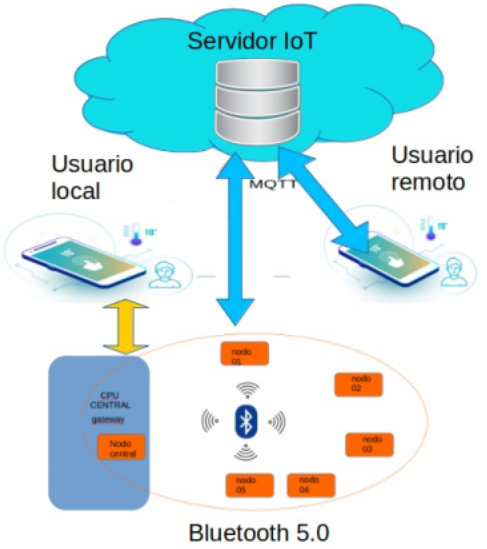
\includegraphics[width=.85\textwidth]{./Figuras/figura1.png}
	\caption{Diagrama en bloques del sistema.}
	\label{fig:diagBloques}
\end{figure}

Esta solución ofrece un mayor control sobre los cultivos, mejora la eficiencia en la gestión del clima y 
optimiza los recursos, lo que se traduce en una mayor productividad y una reducción de los costos operativos.

\section{2. Identificación y análisis de los interesados}
\label{sec:interesados}

En la tabla \ref{tab:interesados}, se pueden identificar los participantes interesados del proyecto.


\begin{table}[ht]
	\begin{tabularx}{\linewidth}{|p{2.15cm}|p{5.8cm}|p{2.85cm}|p{3.4cm}|}
		\hline
		\rowcolor[HTML]{C0C0C0}
		Rol                           & Nombre y Apellido                                                                              & Organización    & Puesto            \\ \hline
		Cliente                       & \clientename                                                                                   & \empclientename & Director Proyecto \\ \hline
		Responsable                   & \authorname                                                                                    & FIUBA           & Alumno            \\ \hline
		\multirow{2}{*}{Orientadores} & \supname                                                                                       & \pertesupname   & Director          \\
		                              & \cosupname                                                                                     & \pertecosupname & Codirectora       \\ \hline
		Opositores                    & \multicolumn{3}{l|}{Empresas que ya ofrecen soluciones similares en el mercado.}                                                     \\ \hline
		Usuario final                 & \multicolumn{3}{l|}{Organizaciones interesadas en la automatización de cultivos en invernaderos.}                                       \\ \hline
	\end{tabularx}
	\caption{Identificación de los interesados.}
	\label{tab:interesados}
\end{table}

\begin{itemize}
	\item Cliente: El \clientename\hspace{1px} es especialista en cultivos y gestión forestal, con amplia experiencia en
	      cultivos hidropónicos. Va a colaborar con la definición de los requerimientos y el seguimiento del proyecto.
	\item Orientadores:
	      \begin{itemize}
		      \item El Director \supname\hspace{1px} es experto en la temática y guiará con la
		            implementación de los protocolos y herramientas del proyecto.
		      \item La Codirectora \cosupname , experta en Sistemas de Información, ayudará con el
		            seguimiento metodológico, para garantizar una gestión rigurosa y efectiva del
		            desarrollo del trabajo.
	      \end{itemize}
\end{itemize}



\section{3. Propósito del proyecto}
\label{sec:proposito}

Diseñar y desarrollar un prototipo preliminar de un conjunto de sensores y
actuadores conectados a través de WiFi, junto con un servidor IoT y
una aplicación web, que permita el monitoreo y control remoto del clima en
invernaderos. El proyecto busca proporcionar a la institución un mayor
control sobre las condiciones ambientales, optimizar el uso de recursos,
reducir los costos operativos y contribuir a una mayor sostenibilidad
ambiental.

\section{4. Alcance del proyecto}
\label{sec:alcance}

El presente trabajo incluye:
\begin{itemize}
	\item Análisis e investigación de ESP-BLE-MESH para microcontroladores ESP32-C3.
	\item Implementación del protocolo ESP-BLE-MESH entre los nodos sensores, actuadores
	      y el nodo central.
	\item Diseño e implementación de la conexión WiFi en el nodo central.
	\item Desarrollo del firmware de los nodos que serán alimentados con fuente 12vcc.
	      \begin{itemize}
		      \item Programación del firmware de los siguentes nodos sensores para la recopilación
		            y transmisión de datos.
		            \begin{itemize}
			            \item Nodo sensor de temperatura ambiente y humedad relativa.
			            \item Nodo sensor de dióxido de carbono ($CO_2$).
			            \item Nodo sensor de potencial de hidrógeno (pH).
			            \item Nodo sensor de conductividad eléctrica (CE).
		            \end{itemize}
		      \item Programación del firmware del nodo actuador de cuatro salidas para gestionar el
		            control de dispositivos y reportar su estado.
		      \item Programación del firmware del nodo central para gestionar la comunicación con
		            los nodos sensores, actuadores y el servidor IoT.
		            \begin{itemize}
			            \item Programación del firmware del ESP32-C3 que actúa como nodo central en la
			                  topología mesh mediante Bluetooth (ESP-BLE-MESH).
			            \item Programación del firmware del ESP32-C3 que opera el servidor web y gestiona la
			                  comunicación con el servidor IoT mediante WiFi.
			            \item Programación del firmware para la comunicación entre los dos ESP32-C3 mediante
			                  UART (\textit{Universal Asynchronous Receiver-Transmitter}).
		            \end{itemize}
	      \end{itemize}
	\item Implementación del broker MQTT en el servidor IoT.
	\item Implementación de cifrados de conexión mediante TLS (\textit{Transport Layer
		      Security}).
	\item Configuración del nodo central para enviar los datos recolectados al servidor
	      IoT mediante el protocolo MQTT.
	\item Diseño e implementación de una base de datos para almacenar los datos
	      recolectados por los sensores y permitir su consulta y análisis.
	\item Diseño y desarrollo de una API (\textit{Application Programming Interface})
	      REST (\textit{Representational State Transfer}) que permita la comunicación con
	      el sistema utilizando HTTP (\textit{Hypertext Transfer Protocol}), MQTT y
	      WebSockets.
	\item Desarrollo de una aplicación Web SPA.
	\item Entrega del código del sistema, que incluye todos los componentes desarrollados
	      (sensores, nodo central, servidor y aplicación web), guías de instalación,
	      configuración y operación.
\end{itemize}

El presente trabajo no incluye:
\begin{itemize}
	\item Diseño de los gabinetes para los nodos sensores, actuadores y nodo central a
	      utilizar.
	\item Desarrollo de una aplicación móvil compatible con iOS y Android.
	\item Desarrollo de módulos para alimentación con baterías.
\end{itemize}

\section{5. Supuestos del proyecto}
\label{sec:supuestos}

Para el desarrollo del presente proyecto se supone que:

\begin{itemize}
	\item Se contará con los materiales necesarios para la implementación de los nodos de
	      sensores, actuadores, como así también del nodo central.
	\item Se contará con el apoyo financiero del cliente para comprar los componentes
	      adicionales necesarios para el desarrollo del prototipo.
	\item Se dispondrá del conocimiento necesario para la implementación del protocolo
	      BLE Mesh en los microcontroladores.
	\item Se dispondrá del conocimiento necesario para la implementación del protocolo de
	      cifrado TLS y el software necesario en los microcontroladores y servidor IoT.
	\item Se dispondrá del conocimiento necesario para el diseño y desarrollo de la base
	      de datos, API y la aplicación SPA.
	\item El cliente tendrá disponibilidad para atender las consultas.
	\item Los directores tendrán disponibilidad para atender las consultas.
	\item Se podrá terminar el presente proyecto en el tiempo estipulado.
\end{itemize}

\section{6. Requerimientos}
\label{sec:requerimientos}

\begin{enumerate}
	\item Requerimientos de los nodos sensores:
	      \begin{enumerate}
		      \item Cada nodo deberá contar con un microcontrolador ESP32-C3.
		      \item Cada nodo deberá conectarse a una red Wi-Fi.
		      \item Cada nodo deberá tener un identificador único dentro del sistema.
		      \item Cada nodo deberá permitir configurar el tiempo de manera remota para enviar los datos recolectados.
		      \item Cada nodo, según corresponda, deberá enviar al servidor IoT:
		            \begin{enumerate}
			            \item la temperatura del ambiente, humedad relativa, presión atmosférica y nivel de luminosidad,
			            \item el nivel de dióxido de carbono,
			            \item el nivel de pH, CE y TDS,
			            \item el nivel y temperatura de la solución nutritiva,
			            \item y consumo de agua, nutrientes y energía eléctrica.
		            \end{enumerate}
	      \end{enumerate}

	\item Requerimientos del nodo actuador:
	      \begin{enumerate}
		      \item Deberá contar con un microcontrolador ESP32-C3.
		      \item Cada nodo deberá conectarse a una red Wi-Fi.
		      \item Deberá tener un identificador único dentro del sistema.
		      \item Deberá contar con cuatro canales.
		      \item Deberá enviar al servidor IoT el estado de cada canal.
		      \item Deberá permitir activar cada canal de manera remota.
	      \end{enumerate}

	\item Requerimientos asociados al Broker MQTT:
	      \begin{enumerate}
		      \item Deberá contar con un broker MQTT que soporte conexiones seguras mediante TLS.
		      \item Deberá gestionar las suscripciones y publicaciones de los datos enviados desde
		            los nodos y permitir la comunicación bidireccional para el envío de comandos.
		      \item Deberá implementar QoS (\textit{Quality of Service}) para garantizar la entrega de los mensajes.
	      \end{enumerate}

	\item Requerimientos asociados al Frontend:
	      \begin{enumerate}
		      \item La interfaz deberá ser intuitiva y accesible desde dispositivos móviles y de escritorio.
		      \item Deberá permitir el acceso al sistema a usuarios debidamente autenticados.
		      \item Deberá permitir realizar el CRUD (\textit{Create, Read, Update and Delete}) de ambientes.
		      \item Deberá permitir realizar el CRUD de sensores asociados a un determinado ambiente.
		      \item Deberá permitir realizar el CRUD de actuadores asociados a un determinado ambiente.
		      \item Deberá permitir visualizar en tiempo real los datos recibidos de los nodos sensores.
		      \item Deberá permitir enviar comandos y configuraciones a los nodos sensores y actuadores.
		      \item Deberá permitir visualizar los datos históricos de los sensores y actuadores.
	      \end{enumerate}

	\item Requerimientos asociados al Backend y la API:
	      \begin{enumerate}
		      \item Deberá permitir conexiones seguras mediante TLS.
		      \item Deberá soportar los métodos HTTP para realizar operaciones CRUD y visualizar los reportes, WebSockets
		            para la visualización en tiempo real de los datos y MQTT para la interacción con los nodos.
			  \item Deberá poder persistir la información de los usuarios.
			  \item Deberá poder persistir la información de los ambientes.
			  \item Deberá poder persistir la información de los sensores.
			  \item Deberá poder persistir la información de los actuadores.
			  \item Deberá poder persistir la información histórica de las mediciones de los sensores.
			  \item Deberá poder persistir la información histórica de los estados de los actuadores.
			  \item Deberá poder persistir la información histórica de los parámetros enviados a los sensores.
			  \item Deberá poder persistir la información histórica de los parámetros enviados a los actuadores.
		      \item Deberá permitir la autenticación y autorización de usuarios autorizados para acceder a los recursos.
		      \item Deberá incluir los endpoints para permitir realizar el CRUD de usuarios para el acceso seguro al sistema.
		      \item Deberá incluir los endpoints para permitir realizar el CRUD de ambientes.
		      \item Deberá incluir los endpoints para permitir realizar el CRUD de sensores asociados a un determinado ambiente, 
			  con la configuración de sus parámetros específicos.
		      \item Deberá incluir los endpoints para permitir realizar el CRUD de actuadores asociados a un determinado ambiente, 
			  con la configuración de sus parámetros específicos por canales.
		      \item Deberá incluir el endpoint para registrar las mediciones de los sensores.
		      \item Deberá incluir el endpoint para registrar los estados de los actuadores.
		      \item Deberá incluir el endpoint para obtener el histórico de las mediciones de los sensores.
		      \item Deberá incluir el endpoint para obtener el histórico de los estados de los actuadores.
		      \item Deberá incluir un endpoint para el envío de parámetros a los sensores.
		      \item Deberá incluir un endpoint para el envío de parámetros a los actuadores.
	      \end{enumerate}

	\item Requerimientos de documentación:
	      \begin{enumerate}
		      \item Se entregará el código del sistema, que incluye todos los componentes desarrollados (sensores, actuadores, Broker MQTT, Frontend, Backend y API).
		      \item Se entregarán las guías de instalación, configuración y operación.
		      \item Se desarrollará un informe de avance al finalizar el Taller de Trabajo Final A.
		      \item Se desarrollará la memoria del proyecto al finalizar el Taller de Trabajo Final B.
	      \end{enumerate}
\end{enumerate}


\section{7. Historias de usuarios (\textit{Product backlog})}
\label{sec:backlog}

Para definir las historias de usuario y estimar su dificultad, complejidad y riesgo, es necesario primero descomponer los requerimientos en historias de
usuario específicas. A cada historia se le asignan puntos de acuerdo con la serie de Fibonacci (1, 2, 3, 5, 8, 13, 21, 34, etc.), que representan los niveles
de dificultad, complejidad y riesgo.

El puntaje total de cada historia de usuario se calcula con la suma de los valores asignados a estos tres criterios, y luego se asigna el número de la
secuencia de Fibonacci más cercano que sea mayor o igual a la suma obtenida. 

Para asignar ponderación a los (\textit{history points}) se han asignado los
siguientes pesos:

\underline{Dificultad del trabajo a realizar}
\begin{itemize}
	\item \textbf{Baja:} Peso \textrightarrow{ 1}.
	\item \textbf{Media:} Peso \textrightarrow{ 3}.
	\item \textbf{Alta:} Peso \textrightarrow{ 5}.
\end{itemize}

\underline{Complejidad del trabajo a realizar}
\begin{itemize}
	\item \textbf{Baja:} Peso \textrightarrow{ 1}.
	\item \textbf{Media:} Peso \textrightarrow{ 5}.
	\item \textbf{Alta:} Peso \textrightarrow{ 13}.
\end{itemize}

\underline{Riesgo del trabajo a realizar}
\begin{itemize}
	\item \textbf{Baja:} Peso \textrightarrow{ 1}.
	\item \textbf{Media:} Peso \textrightarrow{ 3}.
	\item \textbf{Alta:} Peso \textrightarrow{ 5}.
\end{itemize}

\pagebreak

\textbf{Historia de Usuario 1: Desarrollador}
\begin{itemize}
	\item ``Como desarrollador quiero integrar los sensores y actuadores con el sistema para que se comuniquen correctamente a través de la
	      red y asegurar que los datos se transmitan de manera eficiente y segura."

	      \begin{itemize}
		      \item \textbf{Dificultad:} Alta (5) \textrightarrow{ Porque implica múltiples integraciones y la configuración de varios dispositivos para que
			            funcionen en conjunto de manera sincronizada}.
		      \item \textbf{Complejidad:} Alta (13) \textrightarrow{ Porque la integración de todas las tecnologías podría presentar desafíos técnicos}.
		      \item \textbf{Riesgo:} Alta (5) \textrightarrow{ Porque existe incertidumbre sobre posibles problemas de comunicación entre dispositivos
			            y ajustes de la configuración}.
	      \end{itemize}

	      \textit{Story points}= 34.

	      (5 + 13 + 5 = 23 \textrightarrow{ 34}). Es el siguiente valor en la serie de Fibonacci.

\end{itemize}

\textbf{Historia de Usuario 2: Cliente}
\begin{itemize}
	\item ``Como cliente, quiero que el sistema permita la gestión completa de ambientes, sensores y actuadores a través de una interfaz intuitiva,
	      con capacidades para visualizar en tiempo real, ajustar las configuraciones de manera remota y visualizar
	      reportes históricos."

	      \begin{itemize}
		      \item \textbf{Dificultad:} Media (3) \textrightarrow{ Porque implica el desarrollo y personalización de funcionalidades estándar que son comunes
			            en sistemas de monitoreo y control}.
		      \item \textbf{Complejidad:} Alta (13) \textrightarrow{ Si bien existen soluciones de este tipo y se podría consultar a profesionales expertos en la
			            materia, integrar todas las funcionalidades en una interfaz coherente y eficiente podría ser complejo}.
		      \item \textbf{Riesgo:} Media (3) \textrightarrow{ Porque la integración de múltiples módulos y la gestión de datos en tiempo real presenta riesgos
			            moderados que podrían afectar la estabilidad del sistema}.
	      \end{itemize}

	      \textit{Story points}= 21.

	      (3 + 13 + 3 = 19 \textrightarrow{ 21}). Es el siguiente valor en la serie de Fibonacci.

\end{itemize}

\textbf{Historia de Usuario 3: Usuario final}
\begin{itemize}
	\item ``Como usuario final, quiero poder visualizar un panel de control que sea fácil de usar, responsivo desde dispositivos móviles y de escritorio,
	      que me permita gestionar y visualizar datos de sensores y actuadores en tiempo real, además de consultar reportes históricos."

	      \begin{itemize}
		      \item \textbf{Dificultad:} Media (3) \textrightarrow{ Aunque existen herramientas para el desarrollo, la integración de funcionalidades avanzadas
			            y la necesidad de una interfaz de usuario adaptativa para diferentes dispositivos pueden añadir dificultad}.
		      \item \textbf{Complejidad:} Alta (13) \textrightarrow{ El diseño y la implementación de una interfaz responsiva que soporte múltiples funcionalidades
			            (monitoreo en tiempo real, datos históricos, gestión remota) pueden requerir un desarrollo más complejo}.
		      \item \textbf{Riesgo:} Media (3) \textrightarrow{ Si bien existen las tecnologías para desarrollar el proyecto, la implementación exitosa de todas las
			            funcionalidades sin problemas técnicos  y la integración con otras partes del sistema pueden presentar riesgos}.
	      \end{itemize}

	      \textit{Story points}= 21.

	      (3 + 13 + 3 = 19 \textrightarrow{ 21}). Es el siguiente valor en la serie de Fibonacci.

\end{itemize}

\section{8. Entregables principales del proyecto}
\label{sec:entregables}

Los entregables del proyecto son:
\begin{itemize}
	\item Repositorio con:
	      \begin{itemize}
		      \item Código fuente del firmware de los microcontroladores.
		      \item Código fuente de Frontend.
		      \item Código fuente de Backend y la API.
	      \end{itemize}
	\item Diagramas y guías de instalación.
	\item Guías de configuración y operación.
	\item Informe de avance.
	\item Memoria del trabajo final.
	\item Video con demostración del sistema.
\end{itemize}

\section{9. Desglose del trabajo en tareas}
\label{sec:wbs}


\begin{enumerate}
	\item Planificación del proyecto (50 h)
	      \begin{enumerate}
		      \item Elaboración del documento de planificación del proyecto (35 h)
		      \item Diseño de la arquitectura del proyecto (15 h)
	      \end{enumerate}
	\item Investigación preliminar (80 h)
	      \begin{enumerate}
		      \item Investigación de los protocolos MQTT, HTTP y WebSockets (12 h)
		      \item Investigación de certificado TLS (8 h)
		      \item Investigación y elección de los microcontroladores a utilizar (5 h)
		      \item Investigación y elección de los sensores y actuadores a utilizar (10 h)
		      \item Investigación y elección de la base de datos a utilizar (10 h)
		      \item Investigación y elección del framework de backend a utilizar (10 h)
		      \item Investigación y elección del framework de frontend a utilizar (10 h)
		      \item Investigación y elección de la plataforma del servidor IoT a utilizar (10 h)
		      \item Instalación y puesta a punto del entorno de desarrollo (5 h)
	      \end{enumerate}
	\item Prototipado del proyecto (30 h)
	      \begin{enumerate}
		      \item Configuración y conexionado de sensores y actuadores (15 h)
		      \item Integración de componentes y microcontroladores (15 h)
	      \end{enumerate}
	\item Desarrollo del firmware de los microcontroladores (127 h)
	      \begin{enumerate}
		      \item Configuración inicial de los microcontroladores  (2 h)
		      \item Implementación y configuración de los certificados TLS (10 h)
		      \item Implementación del firmware del nodo sensor de temperatura ambiente, humedad relativa, presión atmosférica y nivel de luminosidad (20 h)
		      \item Implementación del firmware del nodo sensor de nivel de dióxido de carbono (15 h)
		      \item Implementación del firmware del nodo sensor de pH, CE y TDS (20 h)
		      \item Implementación del firmware del nodo sensor de nivel y temperatura de la solución nutritiva (20 h)
		      \item Implementación del firmware del nodo sensor de consumo de agua, nutrientes y energía eléctrica (20 h)
		      \item Implementación del firmware del nodo actuador (20 h)
	      \end{enumerate}
	\item Desarrollo del backend (90 h)
	      \begin{enumerate}
		      \item Configuración inicial del entorno (10 h)
			  \item Implementación y configuración de los certificados TLS (10 h)
			  \item Implementación y configuración del broker MQTT (10 h)
		      \item Implementación y configuración de JWT (10 h)
		      \item Implementación y configuración de la base de datos (10 h)
		      \item Implementación y configuración de WebSockets (10 h)
		      \item Implementación de los endpoints de usuarios (4 h)
		      \item Pruebas de los endpoints de usuarios (1 h)
		      \item Implementación de los endpoints de ambientes (2 h)
		      \item Pruebas de los endpoints de ambientes (1 h)
		      \item Implementación de los endpoints de sensores (4 h)
		      \item Pruebas de los endpoints de sensores (1 h)
		      \item Implementación de los endpoints de actuadores (4 h)
		      \item Pruebas de los endpoints de actuadores (1 h)
		      \item Implementación del endpoint de mediciones de sensores (2 h)
		      \item Pruebas del endpoint de mediciones de sensores (1 h)
		      \item Implementación del endpoint de estados de actuadores (2 h)
		      \item Pruebas del endpoint de estados de actuadores (1 h)
		      \item Implementación del endpoint de parámetros enviados a los sensores (2 h)
		      \item Pruebas del endpoint de parámetros enviados a los sensores (1 h)
		      \item Implementación del endpoint de parámetros enviados a los actuadores (2 h)
		      \item Pruebas del endpoint de parámetros enviados a los actuadores (1 h)
	      \end{enumerate}
	\item Desarrollo del frontend (93 h)
	      \begin{enumerate}
		      \item Configuración inicial del entorno (10 h)
		      \item Implementación y configuración de los certificados TLS (10 h)
		      \item Implementación y configuración de JWT (10 h)
		      \item Implementación y configuración de WebSockets (5 h)
		      \item Implementación de la interfaz de login de usuario (4 h)
		      \item Pruebas de la interfaz de login de usuario (1 h)
		      \item Implementación de las interfaces de manejo de usuarios (4 h)
		      \item Pruebas de las interfaces de manejo de usuarios (1 h)
		      \item Implementación de las interfaces de manejo de ambientes (3 h)
		      \item Pruebas de las interfaces de manejo de ambientes (1 h)
		      \item Implementación de las interfaces de manejo de sensores (5 h)
		      \item Pruebas de las interfaces de manejo de sensores (1 h)
		      \item Implementación de las interfaces de manejo de actuadores (5 h)
		      \item Pruebas de las interfaces de manejo de actuadores (1 h)
		      \item Implementación de la interfaz de mediciones de sensores (8 h)
		      \item Pruebas de la interfaz de mediciones de sensores (1 h)
		      \item Implementación de la interfaz de estados de actuadores (8 h)
		      \item Pruebas de la interfaz de estados de actuadores (1 h)
		      \item Implementación de la interfaz de  parámetros enviados a los sensores (3 h)
		      \item Pruebas de la interfaz de parámetros enviados a los sensores (1 h)
		      \item Implementación de la interfaz de parámetros enviados a los actuadores (3 h)
		      \item Pruebas de la interfaz de parámetros enviados a los actuadores (1 h)
		      \item Implementación de la interfaz principal del sistema (5 h)
		      \item Pruebas de la interfaz principal del sistema (1 h)
	      \end{enumerate}
	\item Pruebas y validación (48 h)
	      \begin{enumerate}
		      \item Pruebas de los microcontroladores
		            \begin{enumerate}
			            \item Pruebas de los firmwares de los microcontroladores (5 h)
			            \item Pruebas de conexión y comunicación de los microntroladores (5 h)
			            \item Pruebas de seguridad (5 h)
			            \item Pruebas de sensores y actuadores (5 h)
		            \end{enumerate}
		      \item Pruebas del backend
		            \begin{enumerate}
			            \item Pruebas de MQTT y TLS (3 h)
			            \item Pruebas de validación de almacenamiento de los datos (3 h)
			            \item Pruebas de manejo de los datos en tiempo real y endpoints (3 h)
			            \item Pruebas de seguridad (5 h)
		            \end{enumerate}
		      \item Pruebas del frontend
		            \begin{enumerate}
			            \item Pruebas de interfaz y usabilidad (3 h)
			            \item Pruebas de visualización de los reportes y gráficos (3 h)
			            \item Pruebas de visualización de los datos en tiempo real (3 h)
			            \item Pruebas de seguridad (5 h)
		            \end{enumerate}
	      \end{enumerate}
	\item Documentación del proyecto (97 h)
	      \begin{enumerate}
		      \item Informe de avance (15 h)
		      \item Video con demostración del sistema (2 h)
		      \item Estructura de la memoria del proyecto (10 h)
		      \item Escritura de la memoria del proyecto (40 h)
		      \item Revisión de la memoria del proyecto (10 h)
		      \item Presentación final (20 h)
	      \end{enumerate}
\end{enumerate}



Cantidad total de horas: 615.

\section{10. Diagrama de Activity On Node}
\label{sec:AoN}

\begin{consigna}{red}
	Armar el AoN a partir del WBS definido en la etapa anterior.

	Una herramienta simple para desarrollar los diagramas es el Draw.io
	(\url{https://app.diagrams.net/}). \href{https://app.diagrams.net}{Draw.io}

	\begin{figure}[htpb]
		\centering
		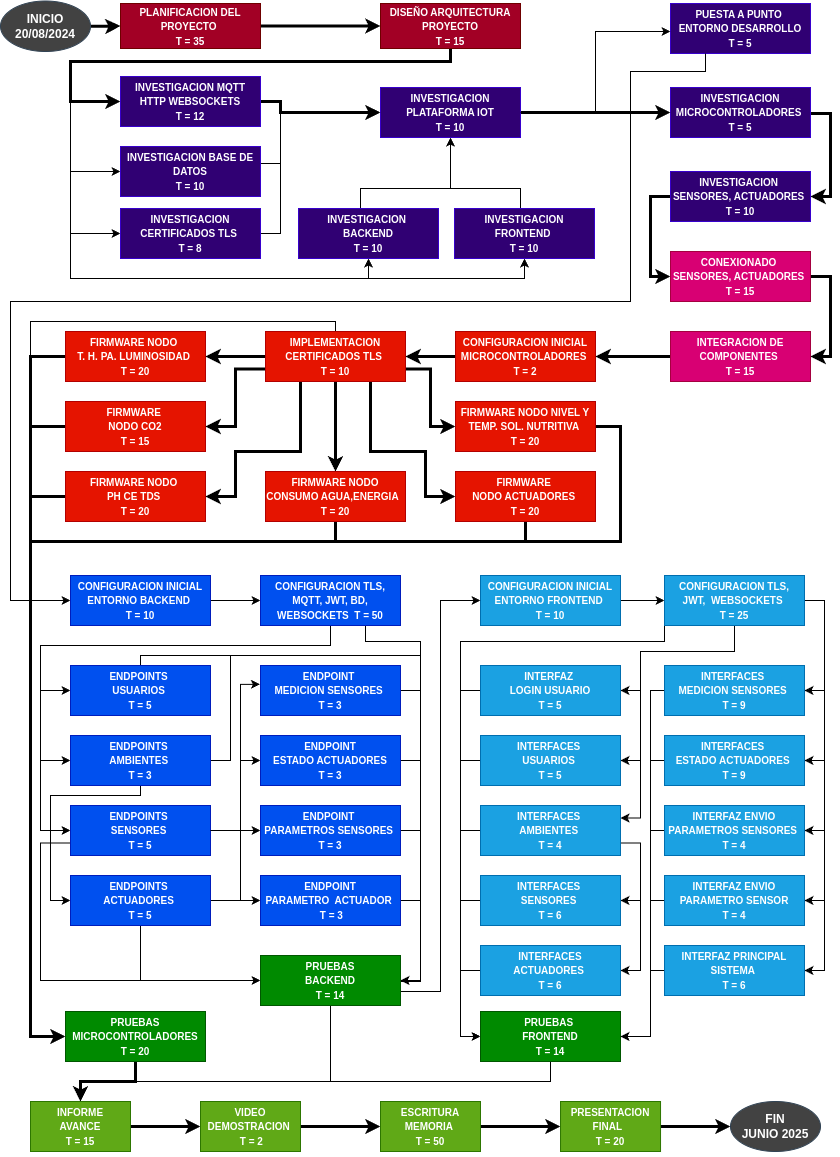
\includegraphics[width=.8\textwidth]{./Figuras/AoN.png}
		\caption{Diagrama de \textit{Activity on Node}.}
		\label{fig:AoN}
	\end{figure}

	Indicar claramente en qué unidades están expresados los tiempos. De ser
	necesario indicar los caminos semi críticos y analizar sus tiempos mediante un
	cuadro. Es recomendable usar colores y un cuadro indicativo describiendo qué
	representa cada color.

\end{consigna}

\section{11. Diagrama de Gantt}
\label{sec:gantt}

\begin{consigna}{red}
	Existen muchos programas y recursos \textit{online} para hacer diagramas de Gantt, entre los cuales destacamos:

	\begin{itemize}
		\item Planner
		\item GanttProject
		\item Trello + \textit{plugins}. En el siguiente link hay un tutorial oficial: \\
		      \url{https://blog.trello.com/es/diagrama-de-gantt-de-un-proyecto}
		\item Creately, herramienta online colaborativa.
		      \\\url{https://creately.com/diagram/example/ieb3p3ml/LaTeX}
		\item Se puede hacer en latex con el paquete \textit{pgfgantt}\\
		      \url{http://ctan.dcc.uchile.cl/graphics/pgf/contrib/pgfgantt/pgfgantt.pdf}
	\end{itemize}

	Pegar acá una captura de pantalla del diagrama de Gantt, cuidando que la letra
	sea suficientemente grande como para ser legible. Si el diagrama queda
	demasiado ancho, se puede pegar primero la ``tabla'' del Gantt y luego pegar la
	parte del diagrama de barras del diagrama de Gantt.

	Configurar el software para que en la parte de la tabla muestre los códigos del
	EDT (WBS).\\ Configurar el software para que al lado de cada barra muestre el
	nombre de cada tarea.\\ Revisar que la fecha de finalización coincida con lo
	indicado en el Acta Constitutiva.

	En la figura \ref{fig:gantt}, se muestra un ejemplo de diagrama de gantt
	realizado con el paquete de \textit{pgfgantt}. En la plantilla pueden ver el
	código que lo genera y usarlo de base para construir el propio.

	Las fechas pueden ser calculadas utilizando alguna de las herramientas antes
	citadas. Sin embargo, el siguiente ejemplo fue elaborado utilizando
	\href{https://docs.google.com/spreadsheets/d/1fBz8NhSpc4tkkhz3KjJCbh1nR_ltDkfEcZi4tZXduqs}{esta
		hoja de cálculo}.

	Es importante destacar que el ancho del diagrama estará dado por la longitud
	del texto utilizado para las tareas (Ejemplo: tarea 1, tarea 2, etcétera) y el
	valor \textit{x unit}. Para mejorar la apariencia del diagrama, es necesario
	ajustar este valor y, quizás, acortar los nombres de las tareas.

	\begin{figure}[htpb]
		\begin{center}
			\begin{ganttchart}[
					time slot unit=day,
					time slot format=isodate,
					x unit=0.038cm,
					y unit title=0.7cm,
					y unit chart=0.6cm,
					milestone/.append style={xscale=4}
				]{2021-03-05}{2021-12-16}
				\gantttitlecalendar*{2021-03-05}{2021-12-16}{year} \\
				\gantttitlecalendar*{2021-03-05}{2021-12-16}{month} \\
				\ganttgroup{Duración Total}{2021-03-05}{2021-12-16} \\
				%%%%%%%%%%%%%%%%%Organización
				\ganttgroup{Organización}{2021-03-05}{2021-04-16} \\
				\ganttbar{Planificación del proyecto}{2021-03-05}{2021-04-15} \\
				%%%%%%%%%%%%%%%%%Ejecución
				\ganttgroup{Ejecución}{2021-04-16}{2021-10-21} \\
				\ganttbar{Tarea 1}{2021-04-16}{2021-04-29} \\
				\ganttbar{Tarea 2}{2021-04-30}{2021-05-13} \\
				\ganttbar{Tarea 3}{2021-05-14}{2021-05-27} \\
				\ganttbar{Tarea 4}{2021-05-28}{2021-07-12} \\
				\ganttbar{Tarea 5}{2021-07-13}{2021-08-09} \\
				\ganttbar{Tarea 6}{2021-08-10}{2021-09-23} \\
				\ganttbar{Tarea 7}{2021-09-24}{2021-09-30} \\
				\ganttbar{Tarea 8}{2021-10-01}{2021-10-14} \\
				\ganttbar{Tarea 9}{2021-10-15}{2021-10-21} \\
				% %%%%%%%%%%%%%%%%%Finalización
				\ganttgroup{Finalización}{2021-10-22}{2021-12-16} \\
				\ganttbar{Memoria v1}{2021-10-22}{2021-11-04} \\
				\ganttbar{Memoria v2}{2021-11-05}{2021-11-18} \\
				\ganttbar{Memoria final}{2021-11-19}{2021-12-02} \\
				% La fecha del siguiente milestone es la fecha en que terminamos la memoria
				\ganttmilestone{Enviar memoria al director}{2021-12-02} \\
				\ganttbar{Elaborar la presentación}{2021-12-03}{2021-12-16} \\
				\ganttmilestone{Ensayo de la presentación}{2021-12-16} \\
				%%%%%%%%%%%%%%%%%%%%%%%%%%%%%%%%%%%%%%%%%%%%%%%%%%%%%%%%%%%%%%%
			\end{ganttchart}
		\end{center}
		\caption{Diagrama de gantt de ejemplo}
		\label{fig:gantt}
	\end{figure}

	\begin{landscape}
		\begin{figure}[htpb]
			\centering
			\includegraphics[height=.85\textheight]{./Figuras/Gantt-2.png}
			\caption{Ejemplo de diagrama de Gantt (apaisado).} %Modificar este título acorde.
			\label{fig:diagGantt}
		\end{figure}

	\end{landscape}

\end{consigna}

\section{12. Presupuesto detallado del proyecto}
\label{sec:presupuesto}

Los precios expresados en la siguiente tabla se encuentran en dólares estadounidenses USD.

\begin{table}[htpb]
	\centering
	\begin{tabularx}{\linewidth}{@{}|X|c|r|r|@{}}
		\hline
		\rowcolor[HTML]{C0C0C0}
		\multicolumn{4}{|c|}{\cellcolor[HTML]{C0C0C0}COSTOS DIRECTOS}   \\ \hline
		\rowcolor[HTML]{C0C0C0}
		Descripción & \multicolumn{1}{c|}{\cellcolor[HTML]{C0C0C0}Cantidad} & 
		\multicolumn{1}{c|}{\cellcolor[HTML]{C0C0C0}Valor unitario} &
		\multicolumn{1}{c|}{\cellcolor[HTML]{C0C0C0}Valor total}\\ \hline
		Mano de obra & 
		\multicolumn{1}{r|}{615} & \multicolumn{1}{r|}{\$25,00} & \multicolumn{1}{r|}{\$15.375,00} \\ \hline
		Cargador celular con cable micro usb & 
		\multicolumn{1}{r|}{6} & \multicolumn{1}{r|}{\$8,40} & \multicolumn{1}{r|}{\$50,40} \\ \hline
		Microcontrolador NodeMCU ESP32 & 
		\multicolumn{1}{r|}{6} & \multicolumn{1}{r|}{\$15,00} & \multicolumn{1}{r|}{\$90,00} \\ \hline
		Caja estanca 90 x 90 x 75 IP65 & 
		\multicolumn{1}{r|}{6} & \multicolumn{1}{r|}{\$3,50} & \multicolumn{1}{r|}{\$21,00} \\ \hline
		Tira de cables de 40 pines Macho Hembra 30 cm & 
		\multicolumn{1}{r|}{3} & \multicolumn{1}{r|}{\$8,15} & \multicolumn{1}{r|}{\$24,45} \\ \hline
		Sensor BME280 3.3V & 
		\multicolumn{1}{r|}{1} & \multicolumn{1}{r|}{\$29,20} & \multicolumn{1}{r|}{\$29,20} \\ \hline
		Sensor Luz Ambiente Lux Bh1750 & 
		\multicolumn{1}{r|}{1} & \multicolumn{1}{r|}{\$6,20} & \multicolumn{1}{r|}{\$6,20} \\ \hline
		Sensor de ($CO_2$) infrarrojo  & 
		\multicolumn{1}{r|}{1} & \multicolumn{1}{r|}{\$95,35} & \multicolumn{1}{r|}{\$95,35} \\ \hline
		Sensor de detección de pH  & 
		\multicolumn{1}{r|}{1} & \multicolumn{1}{r|}{\$94,45} & \multicolumn{1}{r|}{\$94,45} \\ \hline
		Sensor de Conductividad Eléctrica   & 
		\multicolumn{1}{r|}{1} & \multicolumn{1}{r|}{\$69,90} & \multicolumn{1}{r|}{\$69,90} \\ \hline
		Sensor Total de Solidos Disueltos   & 
		\multicolumn{1}{r|}{1} & \multicolumn{1}{r|}{\$29,50} & \multicolumn{1}{r|}{\$29,50} \\ \hline
		Sensor de Distancia Ultrasónico HC-SR04  & 
		\multicolumn{1}{r|}{6} & \multicolumn{1}{r|}{\$3,45} & \multicolumn{1}{r|}{\$20,70} \\ \hline
		Sensor de temperatura sumergible DS18B20  & 
		\multicolumn{1}{r|}{1} & \multicolumn{1}{r|}{\$6,15} & \multicolumn{1}{r|}{\$6,15} \\ \hline
		Módulo de relay de 8 canales  & 
		\multicolumn{1}{r|}{1} & \multicolumn{1}{r|}{\$23,65} & \multicolumn{1}{r|}{\$23,65} \\ \hline
		Válvula solenoide 12V 1/2"  & 
		\multicolumn{1}{r|}{1} & \multicolumn{1}{r|}{\$12,70} & \multicolumn{1}{r|}{\$12,70} \\ \hline
		Caudalímetro 1/2"  & 
		\multicolumn{1}{r|}{1} & \multicolumn{1}{r|}{\$12,55} & \multicolumn{1}{r|}{\$12,55} \\ \hline
		Mini bomba de riego 1/4"  & 
		\multicolumn{1}{r|}{5} & \multicolumn{1}{r|}{\$15,65} & \multicolumn{1}{r|}{\$78,25} \\ \hline
		Caudalímetro 1/4"  & 
		\multicolumn{1}{r|}{5} & \multicolumn{1}{r|}{\$8,45} & \multicolumn{1}{r|}{\$42,25} \\ \hline
		Medidor Energía Monofásico PZEM-004T  & 
		\multicolumn{1}{r|}{1} & \multicolumn{1}{r|}{\$70,00} & \multicolumn{1}{r|}{\$70,00} \\ \hline
		
		%Subtotal
		\multicolumn{3}{|c|}{SUBTOTAL} & \multicolumn{1}{r|}{\$16.151.70} \\ \hline
		\rowcolor[HTML]{C0C0C0}
		\multicolumn{4}{|c|}{\cellcolor[HTML]{C0C0C0}COSTOS INDIRECTOS} \\ \hline
		\rowcolor[HTML]{C0C0C0}
		Descripción                                                 &
		\multicolumn{1}{c|}{\cellcolor[HTML]{C0C0C0}Cantidad}       &
		\multicolumn{1}{c|}{\cellcolor[HTML]{C0C0C0}Valor unitario} &
		\multicolumn{1}{c|}{\cellcolor[HTML]{C0C0C0}Valor total}        \\ \hline
		40\% de los costos directos   & 
		\multicolumn{1}{r|}{1} & \multicolumn{1}{r|}{\$6.460,68} & \multicolumn{1}{r|}{\$6.460,68} \\ \hline
		
		%Subtotal
		\multicolumn{3}{|c|}{SUBTOTAL}                              &
		\multicolumn{1}{r|}{\$6.460,68}                                           \\ \hline
		\rowcolor[HTML]{C0C0C0}
		\multicolumn{3}{|c|}{TOTAL}                                 & \$22.612,38
		\\ \hline
	\end{tabularx}%
\end{table}

\vspace{5mm}
El costo total del proyecto asciende a \textbf{ARS \$22.205.357,16}. Siendo \textbf{\$982,00} el valor del dólar según cambio oficial del 18 de septiembre de 2024.

\section{13. Gestión de riesgos}
\label{sec:riesgos}

\textbf{Definición de riesgos.}

Riesgo 1 - Imposibilidad de cumplir con los plazos establecidos.
\begin{itemize}
	\item Severidad (S): 9.\\ Un retraso en el cronograma afectaría la entrega final del
	      proyecto y podría comprometer su éxito.
	\item Ocurrencia (O): 5.\\ El responsable tiene múltiples compromisos laborales,
	      académicos y familiares, lo que limita el tiempo disponible para dedicarse al
	      proyecto de forma continua.
\end{itemize}

Riesgo 2 - Retraso en la disponibilidad de los componentes para desarrollar el
prototipo.
\begin{itemize}
	\item Severidad (S): 7.\\ La falta de materiales en el tiempo establecido podría
	      retrasar la construcción, programación y prueba del prototipo, lo que afectaría
	      los plazos establecidos para completar el proyecto.
	\item Ocurrencia (O): 5.\\ Existe una posibilidad moderada de que los proveedores no
	      entreguen los materiales a tiempo, por demoras logísticas o problemas de
	      stock, debido a la dependencia de insumos específicos para el prototipo.
\end{itemize}

Riesgo 3 - Selección inadecuada de actuadores, sensores y microcontroladores.
\begin{itemize}
	\item Severidad (S): 8.\\ La elección incorrecta de estos componentes puede generar
	      fallos en el funcionamiento o necesidad de adquirir nuevos dispositivos, lo que
	      causaría retrasos significativos en el desarrollo y pruebas del proyecto,
	      además de incrementar los costos.
	\item Ocurrencia (O): 4.\\ Dado que el proyecto implica el uso de nuevas tecnologías
	      y el responsable no posee experiencia con algunos de estos componentes, existe
	      un riesgo moderado de que la selección inicial no sea la más adecuada.
\end{itemize}

Riesgo 4 - Falta de conocimientos adecuados para el desarrollo del proyecto.
\begin{itemize}
	\item Severidad (S): 7.\\ La falta de experiencia puede llevar a errores en el diseño
	      y desarrollo, aumentando el tiempo necesario para completar el proyecto y
	      potencialmente afectar la calidad y funcionalidad del sistema.
	\item Ocurrencia (O): 6.\\ Aunque es posible adquirir los conocimientos necesarios
	      mediante formación y consulta, existe una probabilidad moderada de enfrentar
	      dificultades debido a la curva de aprendizaje y posibles dificultades técnicas.
\end{itemize}

Riesgo 5 - Cambio de trabajo del responsable del proyecto.
\begin{itemize}
	\item Severidad (S): 9.\\ El cambio de trabajo del único responsable del proyecto
	      puede tener un impacto severo en el progreso, debido a que detendría todo el
	      desarrollo y requeriría la búsqueda de un reemplazo o una reestructuración
	      completa del proyecto. Esto puede causar retrasos muy significativos y posibles
	      problemas de continuidad.
	\item Ocurrencia (O): 4.\\ Aunque el cambio de trabajo es una posibilidad real, la
	      probabilidad de que ocurra durante el proyecto puede ser moderada.
\end{itemize}

\pagebreak

\textbf{Tabla de gestión de riesgos.}

El RPN se calcula como \textit{RPN = S x O}

\begin{table}[H]
	\centering
	\begin{tabularx}{\linewidth}{@{}|X|c|c|c|c|c|c|@{}}
		\hline
		\rowcolor[HTML]{C0C0C0}
		Riesgo                                                & S & O & RPN & S* & O* & RPN* \\ \hline
		Imposibilidad de cumplir con los plazos establecidos. & 9 & 5 & 45  & 9  & 4  & 36   \\ \hline
		Retraso en la disponibilidad de los componentes para
		desarrollar el prototipo.                             & 7 & 5 & 35  & -  & -  & -    \\ \hline
		Selección inadecuada de actuadores, sensores y
		microcontroladores.                                   & 8 & 4 & 32  & -  & -  & -    \\ \hline
		Falta de conocimientos adecuados para el desarrollo del
		proyecto.                                             & 7 & 6 & 42  & 7  & 5  & 35   \\ \hline
		Cambio de trabajo del responsable del proyecto.       & 9 & 4 & 36  & -  & -  & -    \\ \hline
	\end{tabularx}%
\end{table}

\textbf{Criterio adoptado:}

Se tomarán medidas de mitigación en los riesgos cuyos números de RPN sean
mayores a 40.

Nota: los valores marcados con (*) en la tabla corresponden luego de haber
aplicado la mitigación.

\textbf{Plan de mitigación de los riesgos que originalmente excedían el RPN máximo
	establecido.}

Riesgo 1 - Imposibilidad de cumplir con los plazos establecidos.
\begin{itemize}
	\item Planes de mitigación:\\
	      \begin{itemize}
		      \item Establecer hitos intermedios:\\ Dividir el proyecto en fases más pequeñas con
		            fechas límite claras. Esto permitirá monitorear el progreso de manera más
		            efectiva y detectar posibles retrasos a tiempo.
		      \item Implementar un sistema de seguimiento y control:\\ Utilizar herramientas de
		            gestión de proyectos para monitorear el avance del proyecto en tiempo real y
		            detectar desviaciones o retrasos del plan.
	      \end{itemize}
	\item Severidad (S*): 9.\\ La severidad se mantiene constante, pero baja la probabilidad de ocurrencia.
	\item Probabilidad de ocurrencia (O*): 4.\\ Aunque sigue siendo moderada, debido a que
	      el responsable del proyecto sigue teniendo múltiples compromisos, la
	      probabilidad se ajusta para reflejar una disminución considerable en el riesgo,
	      gracias a las medidas proactivas.
\end{itemize}

\pagebreak

Riesgo 4 - Falta de conocimientos adecuados para el desarrollo del proyecto.
\begin{itemize}
	\item Planes de mitigación:\\
	      \begin{itemize}
		      \item Formación continua y capacitación:\\ Realizar cursos especializados en las
		            áreas clave del proyecto, como desarrollo de sistemas embebidos, backend y
		            frontend para asegurar un conocimiento profundo y estructurado.
		      \item Asesoramiento y mentoría:\\ Contactar a expertos o mentores en el campo para
		            recibir orientación y consejos técnicos. Unirse a comunidades o foros
		            especializados para intercambiar experiencias y obtener ayuda con problemas
		            específicos.
	      \end{itemize}
	\item Severidad (S*): 7.\\ La severidad se mantiene constante, pero baja la probabilidad de ocurrencia.
	\item Probabilidad de ocurrencia (O*): 5.\\ La probabilidad de enfrentar dificultades
	      debido a la curva de aprendizaje se reduce con la formación continua y la
	      asesoría. Sin embargo, la curva de aprendizaje y los problemas técnicos pueden
	      aún presentar desafíos, pero la probabilidad de que estos problemas afecten
	      significativamente el proyecto disminuye con un enfoque proactivo.
\end{itemize}

\section{14. Gestión de la calidad}
\label{sec:calidad}

Listado de requerimiento críticos con sus acciones de verificación y
validación:

\begin{itemize}
	\item Requerimientos asociados a los sensores y actuadores:
	      \begin{itemize}
		      \item Req \#1:\\ 1.2. Cada nodo deberá implementar certificados TLS.
		            \begin{itemize}
			            \item Verificación: se realizarán pruebas para asegurar que la comunicación entre los
			                  nodos y el servidor es encriptada y segura.
			            \item Validación: se comprobará que todas las conexiones con el microcontrolador
			                  utilicen certificados TLS.
		            \end{itemize}
		      \item Req \#2: \\ 1.5. Cada nodo deberá permitir configurar de manera remota el
		            tiempo para enviar los datos recolectados.
		            \begin{itemize}
			            \item Verificación: se realizarán pruebas funcionales de la interfaz de configuración
			                  para ajustar el tiempo de envío de datos.
			            \item Validación: se comprobará que se pueda configurar el tiempo de envío de datos
			                  para cada nodo y que los datos sean recolectados y enviados de acuerdo con el
			                  intervalo configurado.

		            \end{itemize}
		      \item Req \#3: \\ 1.6. Cada nodo deberá enviar al servidor IoT los datos
		            recolectados.
		            \begin{itemize}
			            \item Verificación: se realizarán pruebas unitarias para verificar que los datos
			                  enviados por cada sensor son correctos y completos.
			            \item Validación: se realizarán comparaciones de los valores obtenidos por los
			                  sensores con instrumentos de medición de la magnitud correspondiente. Esto
			                  permitirá verificar la precisión de los datos proporcionados por los sensores.
		            \end{itemize}
		      \item Req \#4: \\ 2.6. Cada nodo actuador deberá permitir configurar de manera remota
		            los parámetros del actuador y cada canal.
		            \begin{itemize}
			            \item Verificación: se realizarán pruebas funcionales de la interfaz de configuración
			                  de los actuadores y sus canales.
			            \item Validación: se comprobará que se activan y controlan los canales del actuador y
			                  se verificará su funcionamiento.
		            \end{itemize}
	      \end{itemize}

	\item Requerimientos asociados al Frontend:
	      \begin{itemize}
		      \item Req \#5:\\ 4.1. La interfaz deberá ser intuitiva y accesible desde dispositivos
		            móviles y de escritorio.
		            \begin{itemize}
			            \item Verificación: se realizarán pruebas de usabilidad y compatibilidad en
			                  diferentes dispositivos (móviles, tablets, portátiles y computadoras de
			                  escritorio) para asegurar que la aplicación se visualice correctamente, se
			                  verificará la responsividad y el funcionamiento adecuado de cada componente.
			            \item Validación: se comprobará que todas las secciones de la aplicación son fáciles
			                  de usar y se visualizan correctamente en diversos dispositivos, para confirmar
			                  que la experiencia de usuario sea la adecuada.
		            \end{itemize}
		      \item Req \#6: \\ 4.6. Deberá permitir visualizar en tiempo real los datos recibidos
		            de los sensores y actuadores.
		            \begin{itemize}
			            \item Verificación: se llevarán a cabo pruebas de funcionalidad para asegurar que la
			                  interfaz muestra los datos en tiempo real de manera precisa y continua.
			            \item Validación: se solicitará feedback a los usuarios para verificar que la
			                  visualización de los datos en tiempo real es clara y concisa.
		            \end{itemize}
		      \item Req \#7: \\ 4.7. Deberá permitir enviar comandos y configuraciones a los
		            sensores y actuadores.
		            \begin{itemize}
			            \item Verificación: se realizarán pruebas funcionales de envío de comandos desde la
			                  interfaz y confirmación de la ejecución correcta.
			            \item Validación: se realizarán pruebas de campo para confirmar que los comandos se
			                  ejecutan de manera correcta.
		            \end{itemize}
		      \item Req \#8: \\ 4.8. Deberá permitir la visualización de los datos históricos de
		            los sensores y actuadores.
		            \begin{itemize}
			            \item Verificación: se realizarán pruebas para asegurar que la interfaz muestre
			                  correctamente los datos históricos de sensores y actuadores, comprobar que los
			                  filtros de búsqueda, la navegación entre fechas y la presentación de los datos
			                  funcionen adecuadamente.
			            \item Validación: se solicitará al cliente y usuarios que revisen la interfaz
			                  y proporcionen retroalimentación sobre la utilidad, accesibilidad y claridad de
			                  la visualización de los datos históricos.
		            \end{itemize}
		      \item Req \#9: \\ 4.9. Deberá permitir la visualización en tiempo real y el control
		            de los sensores y actuadores a través de un tablero interactivo.
		            \begin{itemize}
			            \item Verificación: se desarrollarán diferentes tipos de visualizaciones (como
			                  gráficos, tablas, etc.) en el tablero interactivo para asegurar que
			                  proporcionen información clara y efectiva. Se evaluará si permiten una
			                  visualización y control eficiente de los sensores y actuadores.
			            \item Validación: se recogerá retroalimentación de clientes y usuarios para
			                  confirmar que el tablero interactivo es funcional, intuitivo y proporciona una
			                  visión general clara del sistema.
		            \end{itemize}
	      \end{itemize}

	\item Requerimientos asociados al Backend:
	      \begin{itemize}
		      \item Req \#10:\\ 5.1. Deberá permitir conexiones seguras mediante TLS.
		            \begin{itemize}
			            \item Verificación: se realizarán pruebas de seguridad y revisión de las bibliotecas
			                  utilizadas para asegurar que la comunicación es encriptada y segura.
			            \item Validación: se comprobará que todas las conexiones utilicen TLS a través de la
			                  ejecución de requests a todos los endpoints disponibles.
		            \end{itemize}
		      \item Req \#11: \\ 5.2. Deberá poder implementar JWT (JSON Web Token) para poder
		            propagar entre dos partes, y de forma segura, la identidad de un determinado
		            usuario.
		            \begin{itemize}
			            \item Verificación: se realizarán pruebas de integración para confirmar que el
			                  sistema puede generar y validar tokens JWT correctamente. Se verificarán
			                  aspectos como la encriptación del token, su expiración, y la transmisión de la
			                  identidad del usuario entre el cliente y el servidor. También se revisará que
			                  el proceso de autenticación y autorización basado en JWT funciona según lo
			                  especificado.
			            \item Validación: se comprobará que el sistema proporciona una autenticación segura y
			                  que el manejo de los tokens JWT cumple con los requisitos de seguridad y
			                  funcionalidad esperados.
		            \end{itemize}
		      \item Req \#12: \\ 5.3. Deberá soportar los métodos HTTP para realizar operaciones
		            CRUD y visualizar los reportes, WebSockets para la visualización en tiempo real
		            de los datos y MQTT para la interacción con los sensores y actuadores.
		            \begin{itemize}
			            \item Verificación: se realizarán pruebas de funcionalidad para asegurar que los
			                  métodos HTTP (GET, POST, PUT, DELETE) funcionan correctamente para las
			                  operaciones CRUD y la generación de reportes. Se comprobará la implementación
			                  de WebSockets para asegurar que la visualización en tiempo real de los datos es
			                  precisa. Además, se evaluará la comunicación MQTT para verificar que los
			                  mensajes se envían y reciben adecuadamente entre el servidor y los
			                  sensores/actuadores.
			            \item Validación: se comprobará que los métodos HTTP, WebSockets y MQTT cumplen con
			                  las expectativas en términos de desempeño y funcionalidad.
		            \end{itemize}
		      \item Req \#13: \\ 5.8. Deberá poder persistir la información histórica de las
		            mediciones de los sensores.
		            \begin{itemize}
			            \item Verificación: se realizarán pruebas de almacenamiento y recuperación de datos
			                  para verificar que la información histórica de las mediciones de los sensores
			                  se guarda correctamente en la base de datos.
			            \item Validación: se comprobará que la persistencia de la información histórica es
			                  adecuada y accesible para consultas futuras.
		            \end{itemize}
	      \end{itemize}
\end{itemize}

\pagebreak



\section{15. Procesos de cierre}
\label{sec:cierre}

Al finalizar el proyecto, se realizarán las siguientes actividades que permita
una evaluación del proyecto:

\begin{itemize}
	\item Análisis de las pautas de trabajo:
	      \begin{itemize}
		      \item Responsable: \authorname 
		      \item Procedimiento: se realizará una revisión del Plan de Proyecto para:
		            \begin{itemize}
			            \item Verificar si se cumplieron los plazos establecidos.
			            \item Verificar si se cumplieron los objetivos del proyecto.
			            \item Verificar si pudieron cumplimentarse y validarse los requerimientos definidos.
		            \end{itemize}
	      \end{itemize}
	\item Identificación de técnicas y procedimientos útiles e inútiles:
	      \begin{itemize}
		      \item Responsable: \authorname
		      \item Procedimiento: se realizará un análisis de los problemas que surgieron y cómo
		            se solucionaron para:
		            \begin{itemize}
			            \item Examinar los problemas que surgieron durante el proyecto y cómo se resolvieron,
			                  con el fin de identificar las técnicas y procedimientos que resultaron
			                  efectivos o ineficaces.
			            \item Documentar los problemas encontrados, las soluciones implementadas y las
			                  técnicas empleadas durante el desarrollo del proyecto.
			            \item Redactar un informe que analice las técnicas y procedimientos utilizados,
			                  destacar las prácticas que resultaron útiles y señalar las áreas de mejora.
			                  Este informe servirá como guía y referencia para la optimización en futuros
			                  proyectos.
		            \end{itemize}
	      \end{itemize}
	\item Acto de cierre:
	      \begin{itemize}
		      \item Responsable: \authorname
		      \item Procedimiento: se llevará a cabo un acto de cierre formal del proyecto, el cual
		            incluirá los siguientes pasos:
		            \begin{itemize}
			            \item Defensa pública del proyecto: se realizará una presentación pública del
			                  proyecto de manera virtual, donde se expondrán los objetivos, resultados y
			                  conclusiones del trabajo. Esta defensa permitirá mostrar los logros alcanzados
			                  y responder a preguntas formuladas por los participantes de la defensa.
			            \item Agradecimientos Formales:
			                  \begin{itemize}
				                  \item Directores del proyecto: se reconocerá y agradecerá el apoyo y la guía brindada
				                        durante el desarrollo del proyecto.
				                  \item Tribunal evaluador: se expresará el agradecimiento por la evaluación crítica y
				                        constructiva que contribuyó al perfeccionamiento del proyecto.
				                  \item Institución: se agradecerá a la institución que facilitó el entorno y los
				                        recursos necesarios para llevar a cabo el proyecto.
				                  \item Colaboradores: se reconocerá el esfuerzo y la contribución de todos los
				                        colaboradores que hicieron posible el éxito del proyecto, así como su
				                        compromiso y dedicación.
				                  \item Docentes y autoridades de la carrera: se dará un agradecimiento a los docentes
				                        y autoridades que proporcionaron apoyo académico y administrativo, y que
				                        jugaron un papel importante en la formación profesional para el desarrollo del
				                        proyecto.
			                  \end{itemize}
		            \end{itemize}
	      \end{itemize}
\end{itemize}

\end{document}